\section{Overview}
\label{review:overview}

This chapter reviews the state-of-the-art in the related research areas. We begin from the introduction of the sketch-based modeling systems, especially the two important methods of producing 3D models: sketching and sculpting. Then we survey the works on mesh deformation and surface reconstruction from cross section curves, which are two fundamental modeling algorithms in the sculpting and sketching operations respectively.


\section{Digital geometry processing}
\label{ch2:sec:dgp}

With the development of 3D scanner techniques, digital geometry has become a new multimedia type after sound, image and video. It has wide applications in the area of engineering manufacturing, digital entertainment (game, movies, etc.), medicine and biology, art history and archeology, architecture design and so on. With the enlargement of its application area, there is a strong need for the processing techniques of digital geometry modeling, structure analysis and data optimization, leading to the emergence of digital geometry processing.

Digital geometry describes 3D objects and uses 3D surfaces as the main representation. Surfaces in 3D space can be divided into the continuous and discrete forms. The continuous surfaces include parametric surfaces, implicit surfaces and subdivision surfaces. The discrete representations of surfaces include mesh and point cloud, and they are the most popular surface representations in digital geometry processing. This is due to their following advantages: they are relatively simple comparing to the continuous forms, both on the descriptions and transfers; they are the basic data types for the rendering of software and hardware; they are the output forms of most acquisition tools (CT, MRI, 3D scanner, etc.) and the inputs to most simulation/analysis tools.

According to the pipeline of modeling, processing, application and transmission, the main research topics of digital geometry processing are stated as follows.

First of all, since the acquisition from 3D scan equipment is point cloud which is quite irregular, the data needs to be processed for further applications. Point-based graphics provides methods of dealing with points directly, including the representation, modeling, processing and rendering of the points. Point-based graphics does not separate geometry and appearance/attributes of an object, and it seems natural for many 3D acquisition systems. Detailed introductions on point-based graphics can be found at~\cite{AGPPSZ04,GM09}.

However since no connectivity or topology information is available in point cloud, mesh is often a more popular and desirable representation. To reconstruct a mesh from point cloud, two main methods are often used: the geometry-based method and implicit surface-based method. The former often uses the triangulation methods while the latter chooses to fit the points with implicit functions. The representative works of surface reconstruction from point cloud include~\cite{LC87,CL96,ABK98,HDDMS92,CBCMFME01}.

Furthermore, since the point cloud data obtained from scanners may contain noise, difficulties will be brought to the surface reconstruction algorithms, leading to the geometric or topological errors of the reconstructed mesh. So mesh repairing is often needed. The geometric errors denote the holes, self-intersections or face overlaps of the mesh surface and the topological errors include the redundant handles, islands or cavities. The methods for mesh repairing include the surface-based methods~\cite{BS95,LP03,GW01} and volume-based methods~\cite{NT03,JT04,ZJH07}.

Since the initially reconstructed mesh is often irregular, optimization techniques are needed to improve its quality. Mesh smoothing is an optimization method of fairing the mesh surface by only adjusting its geometry. It has multiple applications, such as mesh noise removal and multi-resolution analysis. It reduces curvature variations by moving the mesh vertices and is similar to the high frequency elimination in signal processing. Methods of mesh smoothing include the isotropic~\cite{TG95,DMSB99,LTJW07} and anisotropic filtering~\cite{CDR00,BX03,JDD03,SRML07}, and the selection of a proper algorithm should consider both the speed and the quality.

Another method of regularizing the mesh is remeshing, which reconstructs the geometry and connectivity while striving to preserve the original geometry information. There have been methods proposed for remeshing the triangular mesh~\cite{AVDI03,SG03,AMD02} and quadrilateral mesh~\cite{ACDLD03,ML04}. By remeshing we could make a mesh meet our certain requirement (such as equilateral triangles) or represent the geometry better (such as minimize the number of triangles while preserving the sampling precision).

Mesh simplification can reduce the number of vertices, faces and edges while keeping the original geometry as much as possible, so that the model could be rendered and processed on a computer with low performance. Algorithms of mesh simplification include the vertex-collapse~\cite{SZL92,CVMT96}, edge-collapse~\cite{HDDMS93,HH96,LT98}, and face-collapse~\cite{WHST01} methods. Currently the most popular method is the edge-collapse one which has largest degrees of freedom and best simplification effect.

After a regular mesh is constructed, some further editing operations are often needed. One of the most important editing functions is mesh deformation, which deforms a mesh without changing the topology. A detailed review can be found in Chapter~\ref{ch2:sec:deformation}. Based on deformation, some advanced operations are developed, such as morphing, which generates a series of intermediate shapes between a mesh and its deformed shape and deformation transfer, which transfers the existing mesh deformation from one character to another.

Since a mesh is often a two-manifold embedded in 3D space, comparing to images and videos, it does not have a regular parameter domain. This brings difficulties for the efficient processing of 3D meshes. Mesh parameterization studies the one-to-one mapping between a 3D surface and a simpler and more regular 2D parameter domain. Methods on parameterization include the base mesh parameterization, planar parameterization, spherical parameterization and so on. Parameterization has been used in almost each field of digital geometry modeling and processing. A detailed introduction on mesh parameterization can be found at~\cite{HLS07}.

Given an existing model, there have been a lot of methods proposed for calculating and extracting its features~\cite{GE05,CRT04,PWYLH07,OBS04,RVLL08}. Based on these features, some more advanced operations such as mesh segmentation, shape matching and retrieval can be implemented.

Finally after we have reconstructed and processed a mesh, transmission or storage of the mesh is needed. For complex meshes with lots of details, compression is necessary. This involves conversion between meshes and bit streams. Methods have been proposed for the encoding and decoding of meshes~\cite{JR99,SCT03,KSS00,AG05}, by applying the theory of information and coding.

Digital geometry processing is a fast-growing area of research that uses concepts from applied mathematics, computer science and engineering to design efficient algorithms for the acquisition, reconstruction, analysis, manipulation, simulation and transmission of complex 3D models. For all the above mentioned research topics, a developing trend is towards the combination of various interactive techniques and algorithms for a more intelligent and effective processing. Among all the interactive techniques, sketch-based modeling has drawn much attention from scientists and researchers in recent years. We will then give a detailed review of sketch-based modeling in the following section.


%-----------------------------------------------------------------------------------------------------------------
\section{Sketch-based modeling system}\label{ch2:sec:sbim}

Sketch-based modeling is a method of creating 3D models for use in 3D computer graphics applications. Different from traditional methods which implement the 3D modeling through tediously editing geometric primitives, sketch-based modeling allows the user to draw a 2D shape first and then converts it to a 3D object automatically using various modeling algorithms. That is to say, by using some simple strokes or gestures, the user could create and edit a 3D object to a desired shape. It is somehow like the process that an artist/designer creates a product through drawing on the paper using a pen. In fact, it integrates the knowledge from several diverse domains, such as computer graphics, computer vision, human-computer interaction (HCI), and artificial intelligent (AI).

To combine both speed and ease of paper-based sketching with the flexibility of computer systems, the modeling of 3D objects from 2D drawings and the subsequent editing of the 3D models should be as simple and rapid as possible to provide real-time feedback to the user. So it is necessary to develop a user-friendly interface to allow user to sketch directly unrestricted, and to convey their ideas more vividly. This also requires the existing supporting algorithms to be improved fit the new interface and achieve a better performance.

In recent years, a lot of papers on sketch-based modeling have been published~\cite{OSSJ09}, from the pioneer work Teddy~\cite{IMT99}, to the most recent system ILoveSketch~\cite{BBS08}, proposing different kinds of user interfaces and algorithms. Next we will first review the surface representations in sketch-based modeling systems. Then existing works are classified according to various modeling operations and the related techniques.











Pure constructive--sketching, sculpting
sketching: single view (rule-based) or multiview
sculpting: initial, editing operations

Template-based





















%-----------------------------------------------------------------------------------------------------------------
%how each algorithm model the surface from contour will be stated in the next subsection
\subsection{Surface representations}\label{ch2:sec:sbim:representation}

Surface representation is a fundamental problem in sketch-based modeling. It decides the selection of the related techniques or algorithms. Each representation has its own pros and cons that must be weighted to suit the needs of the intended application. Below we will review the different surface representations used in the sketch-based modeling systems.

Parametric surfaces including NURBS patches, surfaces of revolution and rotational blending surfaces are well studied surface representations for 3D models. They can be easily integrated into diverse applications and exported to various modeling softwares. The reconstructed model using parametric surface representations is usually smooth and easy for the control of level of details. Since traditional methods of modeling a parametric surface are quite difficult and inconvenient for novice users, algorithms based on the sketching technique have been proposed~\cite{EHBE97,CSSJ05,SWSJ06,BLP10}. However, converting a 2D sketch into a parametric surface and editing it is somehow complex. Real-time feedback may not be provided for the user, thus interactive editing is difficult to realize. This makes it go against the original intention of sketch-based modeling.

%should be simplified
Subdivision surfaces can be considered as a generalization of spline surfaces~\cite{ZS00}, since they are also controlled by a coarse control mesh. In addition, they can represent surfaces of arbitrary topology. Subdivision surfaces are generated by repeated refinement of control meshes: after each topological refinement step, the positions of the (old and new) vertices are adjusted based on a set of local averaging rules. A careful analysis of these rules reveals that in the limit this process results in a surface of provable smoothness. Recent works~\cite{BHSF09,NKS09} proposed methods of generating the initial control mesh from 2D user drawings. The final generated 3D control mesh would contain as less number of extraordinary vertices as possible and interpolate the input 2D contours.

Meshes are a simple representation that can easily handle general topology. It is also much easier to reconstruct and edit a 3D mesh, so it is an ideal choice for sketch-based modeling systems~\cite{IMT99,IH03,NSAC05,KPG05,KH06,NISA07,ASN07,ZNA07,KSV09}. However, using mesh representations for modeling makes some operations difficult to implement, such as the blending of two objects. Besides, the mesh quality is also an issue. Usually additional surface optimization algorithms need to be implemented to get a visual-pleasant modeling result.

Implicit surfaces have some advantages over other representations, since it is often easy to implement some operations using implicit surfaces, such as blending and boolean operations~\cite{AGB04,AJ03,KHR02}, for which others types of surface representations are not easy to achieve. The reconstructed implicit surfaces are always smooth, providing visual-pleasant appearance. Unfortunately, sketch-based modeling using implicit surfaces have some inevitable shortcomings due to the inherent limitations of implicit surface. For example, if more details are added to the surface, the rendering would become a burden since more calculations are needed for converting it to a mesh or parametric surface. Some features such as sharp edges are quite difficult to define since a lot of constraints are needed. Besides, implicit surfaces cannot give the user intuitive visual feedback, so the grab-and-drag modeling metaphor is precluded. Nevertheless, with careful implementation, the implicit surface could be an efficient surface representation of sketch-based modeling, and also be used as an intermediate representation from which to extract a mesh.

It could be seen that each kind of surface representation has its own pros and cons, so the selection depends on the specific modeling algorithm and the application of the system. Meanwhile, different techniques could be used to avoid its disadvantages and making it more effective.

%-----------------------------------------------------------------------------------------------------------------
\subsection{Model creation}\label{ch2:sec:sbim:creation}

A basic function of the sketch-based modeling system is the creation of 3D objects. The basic task is reconstructing 3D surfaces from the 2D user sketches. According to the dependence of existing template information, the creation techniques could be classified into two categories.

%-----------------------------------------------------------------------------------------------------------------
\subsubsection{Template-based Systems}\label{ch2:sec:sbim:creation:1}
The first category builds 3D objects through learning existing template models and is usually dedicated to some specific application. They are characterized by the fact that they have some \lq\lq{memory}\rq\rq of 3D shapes built in, which guides their interpretation of input sketches. This requires the analysis of the geometric or semantic features of the template shapes, such as the silhouette of the 3D shape under some views, the curvature distributions, etc. The applications of such systems include modeling clothes~\cite{TWBCH07}, trees~\cite{TST06,OOI06}, hair~\cite{WBC07}, clouds~\cite{WBC08}, architectural shapes~\cite{SketchUp} and so on.

Funkhouser et al.~\cite{FMKCHDJ03} proposed a method of constructing an object using the projected contours of existing models from up to 13 different viewpoints. Object templates are first created by applying image-based transformations to each of the projected contours to extract the fixed-length and rotation-invariant features. Input curves are then matched to an object by applying the same image transformations and comparing against the stored templates. This methods works well for models with simple shapes. However for relatively complex models, the contour information would not be enough to describe the shapes, leading to the errors of the reconstruction result, and it may also become quite tedious for the user to depict the shape of the model they want to build.

The Magic Canvas system~\cite{SI07} uses template retrieval for scene construction. It extracts several contours from each template object and uses a Fourier-based method for sketch matching. It enables the automatic rotation and scaling of the objects to match the input sketch orientation and the inferring of simple geometric relationships. User intervention is required to initiate the retrieval process on sub-sketches within the scene, and also to choose appropriate objects among several candidates.

Yang et al.~\cite{YSM05} propose a similar template-based system, but rather than mesh-based templates, they use procedurally described models. For example, instead of having a mug's mesh for a template, they have a template that describes how to make a mug from simple primitives. This method has the benefit of allowing the template to be deformed to match the input sketch, rather than just replaced with an instance of the template. However, the procedural template definition makes adding new templates more difficult than mesh-base approaches.

Vladislav et. al~\cite{KSV09} present a method of building a 3D model based on an existing template model, shown in Figure~\ref{fig:ModelingFromCtrDraw}. After the template is posed in the scene, the user draws some contours of the new desired model. The input strokes are then aligned and matched with the corresponding feature lines on the template using the Hidden Markov Model algorithm~\cite{LR89}. The final model is constructed by deforming the template using the mean-value encoding algorithm~\cite{KS06}.

\begin{figure} [htbp]
  \centering
  \subfigure[]{
    \centering
    \label{fig:ModelingFromCtrDraw:a} %% label for first subfigure
    \begin{minipage}[b]{0.25\textwidth}
      \centering
      \includegraphics[scale=0.6]{figs/f2.ModelingFromCtrDraw1.eps}
    \end{minipage}}
  \subfigure[]{
    \centering
    \label{fig:ModelingFromCtrDraw:b}
    \begin{minipage}[b]{0.25\textwidth}
      \centering
      \includegraphics[scale=0.6]{figs/f2.ModelingFromCtrDraw2.eps}
    \end{minipage}}
  \subfigure[]{
    \centering
    \label{fig:ModelingFromCtrDraw:c}
    \begin{minipage}[b]{0.25\textwidth}
      \centering
      \includegraphics[scale=0.6]{figs/f2.ModelingFromCtrDraw3.eps}
    \end{minipage}}
  \caption{An example of sketch-based modeling using a given template~\cite{KSV09}. From (a) to (c): a template model, user input contours of the new model and reconstructed new model.}
  \label{fig:ModelingFromCtrDraw} %% label for entire figure
\end{figure}
Although this kind of systems is effective in some specific fields, it is not general or flexible enough, since it largely depends on the richness of the model database and limits user creativity in the sketched scene.

%-----------------------------------------------------------------------------------------------------------------
\subsubsection{Pure Constructive Systems}\label{ch2:sec:sbim:creation:2}

Another category of sketch-based modeling systems is general-purpose shape design. In such kind of systems, the reconstruction of the 3D models from the 2D user input drawings does not need any predefined knowledge, so the ambiguity problem is magnified to some extent. Thus some rules must be followed for the reconstruction of the 3D object from 2D sketches.

In 2000 Hoffman~\cite{HD00} proposed 10 rules for the understanding of a 3D object from the 2D drawings on a paper, from the perspective of visual intelligence. He argued that most people tend to construct a 3D visual world from ambiguous 2D images in conformance to these rules. Among the 10 rules, the following 6 rules are extremely important for the interpretation and reconstruction in pure constructive sketch-based modeling systems:

\begin{enumerate}
	\item[(1)] Always interpret a straight line in an image as a straight line in 3D.
	\item[(2)] If the tips of two lines coincide in an image, then always interpret them as coinciding in 3D.
	\item[(3)] Always interpret lines collinear in an image as collinear in 3D.
	\item[(4)] Always interpret a curve that is smooth in an image as smooth in 3D.
	\item[(5)] Where possible, interpret a curve in an image as the rim of a surface in 3D.
	\item[(6)] Construct surfaces in 3D that are as smooth as possible.
\end{enumerate}

Note that the word \lq\lq{image}\rq\rq in the rules corresponds to the 2D user sketches in sketch-based modeling.

Existing works on the constructive sketch-based modeling systems can be generally divided into 2 categories, according to the specific applications. One is mainly used for the design of engineering systems, which finishes the common Computer-Aided Design (CAD) tasks through sketching; the other aims to build more general objects with free-form shape, which could be used in the initial design step of creating models in computer animation, games and so on.

\textbf{The Engineering Design Systems}: This kind of systems try to design engineering systems with hard edges and rigid corners~\cite{PD92,SG00,CNJC03,PYJH04,FBSS04,VMS05,ML07}, which are similar to the results that a CAD system outputs. The reconstruction of 3D geometry from line drawings is a straightforward and popular method. The fundamental theory and general guidelines for the reconstruction are actually the first three rules proposed by Hoffman.

This issue has been studied in computer vision for some time. Line labeling~\cite{MJ86} is an algorithm of classifying line segments from images as either concave, convex or contour edges, which could be used as the constraints for the reconstruction of the 3D objects. This algorithm could be extended for sketched input by using an stroke-based representation.

A difficulty for such systems is the identification of potential vertices, edges and corners of the 3D objects. In early works this needs to be manually done by the user. For example, Pugh~\cite{PD92} proposed a method of using a basic geometry object such as a cube as a 3D reference, then leaving the work of specifying geometric constraints for the user.	

Later approaches improved it by either implementing the reconstruction incrementally as the user sketches~\cite{CNJC03}, or use some internal rules or vertex-connection templates to create the model after all the complete input sketches~\cite{FBSS04,VMS05}. However, these systems are limited to construct objects consisting of only straight lines, and no curves are allowed.

Varley et al.~\cite{PYJH04} gave an initial attempt on including curves into the sketch-based engineering system design. First of all straight lines are required to create a basic frame of the model, then the user is allowed give some further sketches to modify the shape of the model and let it contain curves. Masry et al.~\cite{ML07} then made this process fully automatic. Their system constructs rigid 3D object consisting of straight lines and curves by using the optimization-based approaches.

\begin{figure} [htbp]
\renewcommand{\thesubfigure}{}
  \centering
  \subfigure[]{
    \centering
    \label{fig:EnginCreation:a} %% label for first subfigure
    \begin{minipage}[b]{0.35\textwidth}
      \centering
      \includegraphics[scale=0.4]{figs/f2.EngCreation1.eps}
    \end{minipage}}
  \subfigure[]{
    \centering
    \label{fig:EnginCreation:b}
    \begin{minipage}[b]{0.35\textwidth}
      \centering
      \includegraphics[scale=0.4]{figs/f2.EngCreation2.eps}
    \end{minipage}}
  \caption{2D sketch and reconstructed 3D model~\cite{ML07}.}
  \label{fig:EnginCreation} %% label for entire figure
\end{figure}

The reconstruction proceeds in two stages: the determination of the depths of the sketch vertices and the reconstruction of the curved strokes. In the first stage, it uses the reconstruction algorithm in an earlier work~\cite{KML04}. It selects a three-connected vertex as the origin and its attached lines as the orthographic projections of the 3D axes. Then the Maximum weight Spanning Tree (MST) algorithm is used to minimize a cost function for the determination of the 3D depth of all the endpoint vertices of all strokes. Similar algorithm is also adopted in~\cite{CCCP04}. Finally by using the gradient steepest descent algorithm, the depth of each curve point can be calculated and thus the curves are straight lines are determined. However in this system the user still has to follow some rules strictly, for example, at least one three-connected vertex must exist. And this sometimes hinders the creativity of the designers. Besides, further modifications are needed to be made if a mechanical object with more details is desired.

The engineering-oriented system provides an efficient way to reconstruct rigid 3D objects. It is to some extent similar to the first category of sketch-based modeling system -- the input strokes are supposed to be the profile curve of the 3D objects -- some prior knowledge is assumed.

\textbf{The Free-form Design Systems}: Although the engineering design systems support curved strokes, the reconstruction is still based on the straight-line representation. Different from this kind of systems, the free-form design systems support the reconstruction of 3D objects from pure curve sketches.

The supporting theories of interpreting and reconstructing 3D objects from curved strokes could be found at the last three rules proposed by Hoffman. The system usually makes the user input curves as smooth as possible and interprets them as contours of the 3D object to be reconstructed. The reconstructed object is also with globally smooth shape.

Following these rules, a common method of reconstruction is to allow the user to sketch a closed curve and build up a smooth 3D model with the input curve as a contour.

The pioneer work Teddy~\cite{IMT99} uses an inflation way to reconstruct a 3D mesh from a user-input closed contour. Similar methods can be found in~\cite{IH01,IH03,NISA07,MI07,NPAI09}. First it samples the closed curve the user inputs to make all edges a predefined unit length. Then it performs constrained Delaunay triangulation of the polygon and some small triangles are merged with the larger ones. Next the chordal axes are obtained by connecting the midpoints of the internal edges. Finally the vertices of the axes are elevated by an amount proportional to their distance from the polygon. This way, a balloon shaped 3D mesh is formed. This method could construct good-looking shapes with few strokes in a short time. The smoothness and quality of the reconstructed mesh are mainly dependent on the related surface optimization and remeshing algorithms.

\begin{figure} [htbp]
  \centering
  \subfigure[]{
    \centering
    \label{fig:Teddy:a} %% label for first subfigure
    \begin{minipage}[b]{0.25\textwidth}
      \centering
      \includegraphics[scale=0.6]{figs/f2.teddy1.eps}
    \end{minipage}}
  \subfigure[]{
    \centering
    \label{fig:Teddy:b}
    \begin{minipage}[b]{0.25\textwidth}
      \centering
      \includegraphics[scale=0.6]{figs/f2.teddy2.eps}
    \end{minipage}}
  \subfigure[]{
    \centering
    \label{fig:Teddy:c}
    \begin{minipage}[b]{0.25\textwidth}
      \centering
      \includegraphics[scale=0.6]{figs/f2.teddy3.eps}
    \end{minipage}}
  \caption{Reconstruction steps in Teddy~\cite{IMT99}. From (a) to (c): preprocessed user input contour, the Chordal axis (bold black lines) and its elevation in 3D space.}
  \label{fig:Teddy} %% label for entire figure
\end{figure}

Olga Karpenko et al.~\cite{KHR02} proposed a similar system to Teddy, but they used the implicit surface instead of mesh as the surface representation of the reconstructed 3D objects. The radial basis function is selected as the implicit function. The system first projects the user-drawn closed curve onto a plane. These projected points then served as the \lq\lq{zero points}\rq\rq, which correspond to the zero value of the basis function. Then each points are displaced slightly along their normal directions to get the \lq\lq {plus points}\rq\rq, which have the values of $1$ of the basis function. By putting all the points and their corresponding values in the equation, the implicit function which represents a blob shape surface is calculated. To make the rendering and some further editing of the model easier, the generated implicit surface is converted to mesh, which interpolates the initial curve that the user draws. Since the implicit surfaces are naturally smooth, no extra surface optimization operations are needed. Besides, for implicit surfaces some further editings such as merging of multiple objects could be easily implemented. Nevertheless the conversion between implicit surface and mesh is inevitable, which may be time-consuming when the shape is complex.

To build surfaces with higher qualities than meshes and implicit surfaces, Nasri et al.~\cite{NKS09} proposed a method of constructing a subdivision surface from user sketched 2D contours. It makes use of the polygonal complex which could converge to a curve under subdivisions to build the surface. The 2D input curves are first preprocessed and sampled to form a closed polygon, using reverse cubic B-spline subdivision algorithm~\cite{BS00}. Then similar method of Teddy~\cite{IMT99} are implemented to partition the polygon and generate the initial 2D control mesh. Next the 3D control mesh is constructed by translating the 2D mesh along two opposite directions. The refined surface which interpolates the initial input 2D curve could finally be built by iterative subdivisions. Different from the above mentioned methods which could build blob-shaped objects, the reconstructed surfaces using this method often suffers from shrinkage, due to the essential characteristics of subdivision surfaces.

A common limitation of these three methods is that all of them are only able to build an object with a simple shape. While in real applications much details are often required to be added. In these systems this mainly rely on the subsequent editing operations of the surfaces.

In order to model an object with some prescribed details directly in the creation phase, CrossSketch~\cite{ASN07} presented a method which constructed one surface with a few strokes in its global shape and small details, by making use of the information of the intersection of strokes. It first classifies the user input curves into hatching strokes which constructs the 3D surface and correlation strokes which give small correlations on the inner shape of the surface. Then it uses the Cubic Corners~\cite{DP1968} to reconstruct the depth of the vertices. A surface with details could be created after the positions of the vertices are calculated. CrossSketch can generate a relatively complex 3D surface with more details while is only able to construct an open surface rather than a closed 3D mesh.

\begin{figure} [htbp]
\renewcommand{\thesubfigure}{}
  \centering
  \subfigure[]{
    \centering
    \label{fig:CrossSketch:a} %% label for first subfigure
    \begin{minipage}[b]{0.35\textwidth}
      \centering
      \includegraphics[scale=0.5]{figs/f2.crosssketch1.eps}
    \end{minipage}}
  \subfigure[]{
    \centering
    \label{fig:CrossSketch:b}
    \begin{minipage}[b]{0.35\textwidth}
      \centering
      \includegraphics[scale=0.5]{figs/f2.crosssketch2.eps}
    \end{minipage}}
  \caption{Reconstruction surface from CrossSketch~\cite{ASN07}.}
  \label{fig:CrossSketch} %% label for entire figure
\end{figure}

Cherlin et al.~\cite{CSSJ05} presented a system which could generate a variety of 3D parametric objects, such as rotational blending surfaces and cross section blending surfaces, with curved and crease features. The quality of the constructed surface is much higher than the systems using other kinds of surface representations. However, the time for constructing objects with relatively complex shapes is usually quite long, making the system unsuitable for interactive modeling applications.

All the above mentioned methods allow the user to input the sketch from just a fixed viewpoint, and this actually impose some limitations on the shape of the reconstructed object. So some methods have been proposed to allow the user to sketch from multiple viewpoints.

Das et al.~\cite{KPG05} showed a system of reconstructing a 3D mesh from curve networks. In this system everytime the user draws a 2D curve, a 3D curve whose normal curvature is the minimum among all the 3D curves whose projections are the 2D curve. This actually parallels with the fourth rule that Hoffman proposed. The user is allowed to draw a network of curves, which formed pieces of surfaces. A 3D object could then be reconstructed by combining all the pieces of surfaces. This system gives the user the flexibility to define the contour of the objects from different viewpoints. However since no references are provided, it is still not an easy task to sketch the satisfactory contours of the object. Besides, it cannot produce meshes with complex topologies.

More recently, Sowel et al.~\cite{SLJGAGL09} proposed a method of reconstructing 3D surfaces from closed curves lying on non-parallel planes. They are mainly applicable to regular defined medical volume data. By manipulating a cutting plane in the 3D data, the user could sketch the intersected contour of the plane and data from the current viewpoints. After a set of contours are sketched, a closed mesh which interpolates them could be created. The reconstruction relies on the predefined volume data, while for sketch-based free-form modeling application, the input strokes may not be regular and analyzing and processing of them may become quite complicated.

Despite all the above mentioned attempts on reconstructing 3D objects from 2D sketches, it is still difficult to create a 3D object with many details with only these creation functions. So subsequent editing operations are also important for modeling a satisfactory object in a sketch-based modeling system. Next we will give a survey on these editing operations.

%-----------------------------------------------------------------------------------------------------------------
\subsection{Augmentation}\label{ch2:sec:sbim:augmentation}

As introduced in the previous section, creating a 3D model from 2D sketches is not a trivial problem whose feasible solutions probably lead to simplistic shapes. Surface augmentation allows user to sketch more features on the surface of the model to create more elaborate details.

Surface augmentation can be thought of as the melding of two surfaces: the original surface and the sketched features. According to the scale of the added feature, surface augmentation could be divided into 3 categories: The big scale feature creation which is carried out on the whole model to augments its general shape, such as surface extrusion; The small scale surface augmentation which focuses on creating detailed features on local parts of the surface; The surface deformation techniques which produce surfaces with appealing shapes without introducing any additional features -- all elements in the final surface come from the original surface.

%mesh extrusion
Teddy~\cite{IMT99} and FiberMesh~\cite{NISA07} have presented an extrusion function for meshes. It is a two-stroke operation: a closed stroke on the surface suggesting the part to extrude and a stroke depicting the silhouette of the extruded surface. The user draws a closed stroke on the object surface and then rotates the model to bring the circle sideways and draws a silhouette line to extrude the surface. This is basically a sweep operation that constructs the 3D shape by moving the closed surface line along the skeleton of the silhouette. The direction of extrusion is always perpendicular to the object surface.

\begin{figure} [htbp]
\renewcommand{\thesubfigure}{}
  \centering
  \subfigure[]{
    \centering
    \label{fig:extrusion:a} %% label for first subfigure
    \begin{minipage}[b]{0.31\textwidth}
      \centering
      \includegraphics[scale=0.7]{figs/f2.extrusion1.eps}
    \end{minipage}}
  \subfigure[]{
    \centering
    \label{fig:extrusion:b}
    \begin{minipage}[b]{0.31\textwidth}
      \centering
      \includegraphics[scale=0.7]{figs/f2.extrusion2.eps}
    \end{minipage}}
  \subfigure[]{
    \centering
    \label{fig:extrusion:c}
    \begin{minipage}[b]{0.31\textwidth}
      \centering
      \includegraphics[scale=0.7]{figs/f2.extrusion3.eps}
    \end{minipage}}
  \caption{Extrusion operation in FiberMesh~\cite{NISA07}.}
  \label{fig:extrusion} %% label for entire figure
\end{figure}

%implicit surface, extrusion
Similarly, the system presented in~\cite{KHR02} allows the user to do extrusion by drawing the original object and the extruded part separately and then combine it either automatically or manually by giving a guidance stroke. Since implicit surface representation is used, the implementation becomes much more easier.

However for the existing extrusion functions provided in the current systems, since the operation is manipulated by the user on a 2D screen and no references are provided in the 3D space, it is difficult to control the relative position and orientation of the extruded part w.r.t. the original model.

%feature creation
Besides extrusion, some systems also provide tools for creating some feature details on the existing model. The systems~\cite{NSAC05,OSSJ05,NISA07} enables the user to create sharp or smooth features on the current mesh, such as sharp creases (Fig~\ref{fig:featurecreation}). The system projects the user drawn stroke onto the existing mesh surface, then the features are created along the projected stroke by moving the related vertices. Usually the direction of the movement is along the normal of each vertex. Furthermore, the projected sketch stroke could be seen as new positional constraints for some advanced surface optimization operations~\cite{NISA07,EP09}. Yotam et al.~\cite{GZ08} enhances the feature creation function by using the shading information. They present a sketch-based modeling system by letting the user draw shadings on a 3D shape directly to create different kinds of features, just like what the artists do when drawing 2D pictures.

\begin{figure} [htbp]
\renewcommand{\thesubfigure}{}
  \centering
  \subfigure[]{
    \centering
    \label{fig:featurecreation:a} %% label for first subfigure
    \begin{minipage}[b]{0.35\textwidth}
      \centering
      \includegraphics[scale=0.6]{figs/f2.featurecreation1.eps}
    \end{minipage}}
  \subfigure[]{
    \centering
    \label{fig:featurecreation:b}
    \begin{minipage}[b]{0.35\textwidth}
      \centering
      \includegraphics[scale=0.6]{figs/f2.featurecreation2.eps}
    \end{minipage}}
  \caption{An example of feature (crease) creation~\cite{NSAC05}.}
  \label{fig:featurecreation} %% label for entire figure
\end{figure}

The third kind of surface augmentation -- the surface deformation techniques, will be reviewed in detail in Chapter~\ref{ch2:sec:deformation}.


%-----------------------------------------------------------------------------------------------------------------
\subsection{Others}\label{ch2:sec:sbim:others}

Like other traditional 3D modeling softwares, sketch-based modeling systems also support many other modeling operations, which make the systems more useful and powerful for various applications.

For example, some mesh cutting algorithms have been proposed to segment an existing model into different meaningful parts. Earlier work~\cite{IMT99,FKSMKTRD04,LLSCS04} used intelligent scissoring tools to cut the mesh. To execute a cut,the user needs to sketch along the cut boundary to specify a sparse set of points. This task could be quite tedious when the cutting boundary is complicated. Some methods were then proposed for fast and easy mesh decomposition~\cite{JLCW06,WPPYM07,MJL08,BMB09}. The user only needs to draw strokes which specify the foreground/background regions for each cut. With this function, it becomes easier analyze and segment a given model so that further modifications could be implemented.

Some operations such as blending~\cite{CSSJ05,WM07}, twisting~\cite{BK04},tunneling(genus creation)~\cite{IMT99,NISA07} and so on are also supported by some sketch-based modeling systems. The availabilities of such functions are closely related to the surface representations and the specific applications of the systems.

Sketch-based modeling systems are especially suitable for quick modeling tasks where exact results are not quite desirable. Like most of other modeling process, it is an iterative process: A rough shape will first be drawn and then various detail modifications are to be made. A hybrid system that contains a substantial shape memory, robust creation rules, and perhaps the ability of continuous learning should be the potential research direction people pursue. Besides, how to apply the sketch-based techniques to other digital geometry processing algorithms to make them more intelligent, is also becoming a useful and popular research topic.


%-----------------------------------------------------------------------------------------------------------------
Mesh deformation: general purpose and special purpose
general: as currently written
special purpose: structure-aware, feature-aware, ...


\section{Surface-based mesh deformation}\label{ch2:sec:deformation}

\subsection{Mesh deformation}\label{ch2:sec:deformation:intro}

As mentioned in Chapter~\ref{ch2:sec:sbim:augmentation}, deformation is an important tool for editing of a created model. The surface deformation methods for parametric or subdivision surfaces have already been developed for years. But these algorithms are difficult to be applied directly to triangular meshes. Due to its importance in various kinds of applications such as geometric modeling and computer animation, mesh deformation has become a popular research topic in digital geometry processing.

There have been abundant researches on mesh deformation, since the early 1980s. Existing methods can be divided into two categories: the space-based deformation~\cite{GB08} and the surface-based deformation~\cite{BS08}.

The space-based deformation methods indirectly reshape an object by warping its surrounding space, with results that are similar to modeling a highly malleable substance. They are computationally efficient and applicable to a variety of object representations. Since manipulating ambient space directly is infeasible, deformations are controlled by tools of various dimensions, such as points~\cite{BK05}, curves~\cite{SF98,PJF97} and volumes~\cite{SP86,JSW05,LLC08}. However in these methods, when large scale deformation happens, the geometric details on a mesh could not be well preserved. Besides, it is not suitable for applications where direct manipulations on the mesh surfaces are needed.

Contrary to spatial deformation, the surface-based methods carry out the mesh deformation by allowing direct manipulation of the mesh surfaces. They can be further classified according to the shape-intrinsic degrees of the representations of the mesh.

The multi-resolution methods~\cite{ZSS97,GSS99,KCVS98,KVS99,SL99,BK04} can be seen as partially surface-intrinsic representations. These methods encode a mesh as a base layer and several levels of refinement, according to its surface geometric properties. The base layer is the low-frequency component of the shape and it is typically represented in Cartesian coordinates. Thus it is not shape-intrinsic, but the shape details are represented in an intrinsic manner: the refinements are described locally, so that the geometric details are mostly captured in a discrete set of translation and rotation-invariant coordinates. Using this representation, modeling operations can be performed on an appropriate user-specified level-of-detail. During the deformation process, only the low-level layers are deformed and the high levels with more details keep fixed, so that the details of the mesh are preserved. The advantage of the multi-resolution approach is the straightforward representation of the details of the shape in a manner that is invariant to the global coordinate system. Nevertheless, in this approach the user needs to explicitly set the required amount of smoothing to create a satisfactory base mesh. In meshes with complex details, many levels of multi-resolution hierarchy may be required to handle the details correctly. Thus it is not appropriate for interactive deformations which require the fast and convenient operations.

The single-resolution method is recognized as pure shape-intrinsic surface-based deformation. Comparing to the above mentioned methods, it has three advantages:

First, it encodes the geometric details of a mesh in some measurements, such as the differential coordinates, which is also called the Laplacian coordinates. Since these measurements are computed by local operators, they naturally contain the local relationship between primitives (usually be vertices) and their one-ring neighbors, and thus are superior to the local displacement representation of mesh details in the multi-resolution method. By preserving these measurements, the mesh details can be well preserved during deformation.

Second, the deformed mesh can often calculated through solving a sparse linear system. By solving the optimization problem in least-squares sense, the caused distortion can be distributed through all the mesh to achieve high-quality deformation result. Moreover, the calculation is real-time by using advanced linear solvers.

Finally, since the measurements are estimated directly on the surface of a mesh, the users could easily implement the deformation by directly manipulating the mesh surfaces, for examples, dragging the vertices on mesh.

The last two advantages make the single-resolution surface-based deformation methods a natural choice for the interactive geometric editing applications, such as the sketch-based modeling.

%-----------------------------------------------------------------------------------------------------------------
\subsection{Continuous mathematical formulation}\label{ch2:sec:deformation:formula}

An intuitive deformation tool should allow the user to easily edit the object and produce a naturally expected deformation result. A natural deformation usually refers to a deformation that behaves like a real-world object, made of physical material. So we start introducing the surface-based method by deriving its mathematical formulations from the physically accurate nonlinear thin shell deformation energy.

Let $S \subset \mathbb{R}^3$ be a two-manifold surface, parameterized by a function $p$ : $\Omega \subset \mathbb{R}^2 \to S \subset \mathbb{R}^3$. This surface is to be deformed to $S^\prime$ by adding to each point $p(u,v)$ a displacement vector $d(u,v)$, such that $S^\prime = p^\prime (\Omega)$ with $p^\prime= p + d$.

It is known from differential geometry~\cite{MPDC76} that the first and second fundamental forms, $\textbf{I}(u,v), \textbf{II}(u,v) \in \mathbb{R}^{2 \times 2}$, can be used to measure geometrically intrinsic (parameterization independent) properties of $S$, such as lengths, areas, and curvatures. The change of fundamental forms therefore yields a measure of stretching and bending energy~\cite{TPBF87}:

\begin{equation}
\label{eq:thinshell}
E_{shell}(S^\prime)= \int_{\Omega}{k_s \Big\|{\textbf{I}^\prime-\textbf{I}}\Big\|_{F}^2+
k_b \Big\|{\textbf{II}^\prime-\textbf{II}}\Big\|_{F}^2 dudv} ,
\end{equation}
where $\textbf{I}^\prime$, $\textbf{II}^\prime$ are the fundamental forms of $S^\prime$, $\left\| \cdot \right\| _F$ denotes a Frobenius norm, and the stiffness parameters $k_s$ and $k_b$ are used to control the resistance to stretching and bending.

Specifically in a deformation task, the user is often allowed to specify the shape of a part of the surface $S^\prime$ to define some boundary constraints. The shape of the other part of $S^\prime$ is then calculated by solving for a surface whose first and second fundamental forms satisfy Eqn~\ref{eq:thinshell}.

However, this nonlinear minimization is computationally too expensive for interactive applications. Hence, it is simplified by replacing the change of first and second fundamental forms by first and second order partial derivatives of the displacement function $d$~\cite{CG91,WW92} :

\begin{eqnarray}
\label{eq:thinshelllinear}
E_{shell}^\prime(d) &=& \int_{\Omega}{k_s \Big( {\left\| {d_u} \right\|}^2 + {\left\| {d_v} \right\|}^2 \Big )}+\nonumber\\
& & k_b \Big( {\left\| {d_{uu}} \right\|}^2 + 2{\left\| {d_{uv}} \right\|}^2 +{\left\| {d_{vv}} \right\|}^2 \Big )dudv ,
\end{eqnarray}
where $d_x=\frac{{\partial d}}{{\partial x}}$ and $d_{xy}=\frac{{\partial^2 d}}{{\partial x}{\partial y}}$ .

The minimization of Eqn~\ref{eq:thinshelllinear} can be efficiently solved by using the Euler-Lagrange PDE function:

\begin{equation}
\label{eq:ELPDE}
	-k_s\Delta d+k_b\Delta^2 d=0,
\end{equation}
where $\Delta d=\texttt{div}\nabla d=d_{uu}+d_{uv}$ is the Laplacian operator and $\Delta^2 d=\Delta(\Delta d)=d_{uuuu}+2d_{uuvv}+d_{vvvv}$ is the bi-Laplacian operator.

The above functions give the way of computing the continuous surface deformation problem. Since a mesh can be regarded as a piecewise linear discrete surface, different methods of discretization are developed.

We next divide the methods into two categories: the linear method and nonlinear method. The former formulates the deformation problem into a linear system that needs to be solved only once, whereas the latter tries to get more precise results through iterative calculations.

%-----------------------------------------------------------------------------------------------------------------
\subsection{Linear methods}\label{ch2:sec:deformation:linear}

The most popular method of discretizing the continuous thin shell energy for triangular meshes is the differential coordinates, which makes the mesh deformation problem a linear one. It is originated from the Laplace-Beltrami operator $\Delta_S=\texttt{div}_S\nabla_S$, which makes the change of second derivatives in Eqn~\ref{eq:thinshelllinear} to closely approximate the change of the curvatures of a continuous surface, by letting the parameterization $\Omega$ equal to the initial surface $S$ itself. As a result, in Eqn~\ref{eq:ELPDE} the Laplacian operator $\Delta$ becomes the Laplace-Beltrami operator $\Delta_S$ and Eqn~\ref{eq:ELPDE} becomes:

\begin{equation}
\label{eq:LBcontin}
	-k_s\Delta_S d+k_b\Delta_S^2 d=0.
\end{equation}

Let $M=(V,E,F)$ be a triangular mesh with $n$ vertices. $V = \{v_i | v_i \in R^3, i = 1,...,n\}$ denotes
the set of vertices, $E = \{e_{ij} = (v_i, v_j) | v_i,v_j \in V, i\ne j\}$ denotes the set of edges, and $F = \{f_{ijk} = (v_i, v_j, v_k) | v_i,v_j,v_k \in V, i\ne j\ne k\}$. Then the discrete Laplace-Beltrami operator defined at each vertex $v_i$ of the mesh is:

\begin{equation}
\label{eq:LBdisc}
\delta_i=D(v_i)=\omega_i \sum\limits_{j\in N(i)}{\omega_{ij} (v_j-v_i)},
\end{equation}
where $N(i)=\{j|e_{ij}\in E\}$ is the index set of adjacent vertices in the \textit{neighboring ring} of vertex $v_i$ and $\omega_{ij}$ is the weight of the edge $e_{ij}$. The \textit{neighboring ring} is also called the 1-ring neighbors. $\delta_i$ here is also called the differential coordinate/Laplacian vector. $\omega_i$ and $\omega_{ij}$ is the corresponding weight~\cite{MDSB02} defined as follows:

\begin{equation}
\label{eq:laplacebetramiweight}
\omega_i=\frac{1}{A_i},\quad \omega_{ij}=\frac{1}{2}(\cot \alpha_{ij}+ \cot \beta_{ij}),
\end{equation}
where $\alpha_{ij}$ and $\beta_{ij}$ are the two angles opposite to the edge ($v_i,v_j$), and $A_i$ is the Voronoi area of vertex $v_i$. An example of the Laplacian vector at a vertex can be seen in Figure~\ref{fig:vertexLaplacian}.

\begin{figure} [htbp]
	\centering
  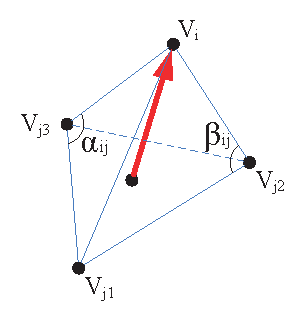
\includegraphics[scale=1]{figs/f2.VertexLaplacian.eps}
  \caption{The Laplacian vector at vertex $v_i$ is the red vector pointing to $v_i$ from the center of its neighbors. $\alpha_{ij}$ and $\beta_{ij}$ are the two angles used for calculating the weight for the edge between $v_i$ and $v_{j1}$.}
  \label{fig:vertexLaplacian} %% label for entire figure
\end{figure}


The Laplacian vector is a shape-intrinsic representation which encodes the local relationship among a vertex and its 1-ring neighborhood. Its magnitude and direction approximate the mean curvature and normal direction at that vertex respectively.

Using Eqn~\ref{eq:LBdisc}, we could represent the mesh geometry using a set of Laplacian coordinates $\Delta=\{\delta_i\}$. For a given mesh $M$, the transformation between $V$ and $\Delta$ could be described through the following equation:

\begin{equation}
\label{eq:simplelaplaciansystem}
LV=\Delta,
\end{equation}
where $L$ is an $n\times n$ coefficient matrix ($n$ denotes the number of vertices) that has the following form:

\begin{numcases}
{L_{ij}=}
\sum\limits_{j \in N(i)}{\omega_{ij}}, & $i = j$\nonumber\\
-\omega_{ij}, & $(i,j) \in E$\nonumber\\
0. & otherwise \nonumber
\end{numcases}

It is noted that $L$ has rank $n-1$, which means $V$ can be recovered from $\Delta$ by fixing one vertex and solving a linear system.

The approach of performing a mesh deformation task using Laplacian coordinates is to designate the new absolute positions $\{c_i\}$ of several vertices (see~\cite{LSCLRS04}), i.e.:

\begin{equation}
\label{eq:lapconstr}
v_i^\prime=c_i ,\quad \quad i\in\{m,...,n\},m<n
\end{equation}
and solve for the remaining vertices $\{v_i^\prime\},i\in \{1,...,m-1\}$ by fitting the new Laplacian coordinates of the deformed mesh to the given Laplacian coordinates of the original mesh. The vertices whose positions are to be designated usually include the \textit{handle} vertices, which the users want to move to designated new 3D locations and the \textit{static} vertices, which are expected to stay fixed during the deformation process. The other vertices whose positions need to be solved are usually called the \textit{Region of Interest} (ROI) vertices.

It has been observed that the solution behaves better if the positional constraints $\{c_i\}$ are satisfied in a least-square sense rather than exactly~\cite{LSCLRS04,SCLARS04}. This results in the following object function

\begin{equation}
\label{eq:laplaciansystemnorotation}
E(V^\prime)=\sum\limits_{i=1}^n {||\delta_i-D(v_i^\prime)||}^2 +
\sum\limits_{i=m}^n {||v_i^\prime-c_i||}^2 ,
\end{equation}
which should be minimized. The new position $v_i^\prime$ of each vertex after deformation could then be obtained by solving a sparse linear system.

The rationale of this method is to preserve the local details of the shape through minimizing the change of the Laplacian vectors during the deformation process. However, it has been mentioned that the Laplacian vector is not invariant under rotation and scale transformations. So if a deformation that contains rotation or scale happens on a given mesh, using the method of Eqn~\ref{eq:laplaciansystemnorotation} will try to preserve the orientation and magnitude of the Laplacian vectors w.r.t. the global coordinate system, whereas in reality these vectors should be rotated or scaled. So the transformations of the Laplacian vectors during the deformation process should be considered. Assume the transformation function for a Laplacian vector $\delta_i$ be $F(\delta_i)$, then the object function which has to be minimized for solving the deformation problem becomes:

\begin{equation}
\label{eq:laplaciansystem}
E(V^\prime)=\sum\limits_{i=1}^n {||F(\delta_i)-D(v_i^\prime)||}^2 +
\sum\limits_{i=m}^n {||v_i^\prime-c_i||}^2 .
\end{equation}

Mesh editing using differential coordinates is first explored by Marx Alexa in~\cite{AM01}. The way he uses is just as in Eqn~\ref{eq:laplaciansystemnorotation}, where $F(\delta_i) = \delta_i$. Since no local transformations were estimated, this approach was only suitable for deformations that do not contain rotation or scaling.

There are some subsequent methods proposed to estimate the transformation of the Laplacian vector. These methods can be classified into implicit and explicit types. The former methods evaluate the transformation according to the deformed surface, whereas the latter methods do not consider the deformed surface at all.

Yu et al.~\cite{YZXSBGS04} proposed an explicit method of propagating the transformation of the handle vertices to the other vertices of the mesh using geodesic interpolation. Besides the positional constraints, the user has to specify the transformation matrix for the handle vertices explicitly. The transformation matrix is then decomposed into rotation and scaling matrices and interpolated over the ROI vertices of the mesh according to their geodesic distances to the handles.

Instead of using geodesic interpolation, Zayer et al.~\cite{ZRKS05} proposed to use the harmonic interpolation, which computes a smooth harmonic scalar filed on the mesh to control the propagation of the transformation. This method shows smoother distributed local transformations and has better result than the geodesic propagation method.

Popa et al.~\cite{PJS05} further generalized the harmonic propagation to material-aware propagation. A stiffness field painted by the user or learned from examples is used to control the weight propagation. They show that physically plausible deformation result can be achieved through proper stiffness filed.

However, all these three methods require manual specification of the transformation at the handles by the user. Moreover, since only rotation and scaling are considered in the transformation, when the handle vertices are only translated, there would be no change of orientation to be propagated. This will lead to the distortion of the local shape features.

Different from the explicit methods, the implicit methods try to estimate the transformation automatically from the unknown vertex positions of the deformed surface.

Lipman et al.~\cite{LSCLRS04} proposed to estimate a local rotation for each vertex between the original mesh and an initial deformation result calculated using Eqn~\ref{eq:laplaciansystemnorotation}. Then the Laplacian vectors are rotated and a new deformed mesh is calculated using these rotated Laplacian vectors. This process is repeated for several iterations until satisfactory result is obtained. This method of estimating the rotation only works well for relatively smooth surfaces with no largely protruding features. Besides, since no scale is considered in the transformation, this approach can not preserve the details under stretching deformations.

Sorkine et al.~\cite{SCLARS04} proposed to explicitly represent the transformation of the Laplacian vectors with a linearized matrix $T_i$, so that $F(\delta_i)=T_i\delta_i$ in Eqn~\ref{eq:laplaciansystem}.
$T_i$ is obtained by estimating the transformation of vertex $v_i$ and its 1-ring neighborhood. By representing $T_i$ as the initial and deformed vertex positions and putting it into Eqn~\ref{eq:laplaciansystem}, the deformed mesh could be calculated. This method works well for deformations with small rotations. However, since rotation in 3D space is actually nonlinear, the linearization of $T_i$ makes it difficult to handle large rotation of the Laplacian coordinates.

To overcome this problem, Fu et al.~\cite{FAT07} use a two-step strategy to estimate the local transformation. Instead of limiting the local transformation $T_i$ to be linearized, this method allows it to be any affine-transformation. In the first step, this method directly solves the local transformation $T_i$ associated at each vertex $v_i$. In order to obtain visual-pleasant deformation result, in the second step, a similarity transformation of $v_i$ is derived from the solved affine-transformations of its neighbors and then used to transform the Laplacian coordinates for the subsequent mesh reconstruction. This approach enables larger rotations than~\cite{SCLARS04}, but it requires tweaking the relative weighting of local transformation smoothness terms; moreover the formulation of implicit transformations may be ill-conditioned for flat one-rings, in which case a perturbation is required. Besides, only isotropic scale is considered in the local transformation, while anisotropic scale often obtains better results.

The Laplacian mesh editing is further generalized to volume graph Laplacian in~\cite{ZHSLBGS05}. This method constructs a graph representing the volume inside the input mesh. The graph Laplacian coordinates encode volumetric details as the difference between each point in the graph and the average of its neighbors. Preserving these volumetric details during deformation imposes a volumetric constraint that prevents unnatural changes in volume. However, the editing requires the construction of the graph and does not fit for the applications that interactive manipulation of the mesh surface is desired.

Nealen et al.~\cite{NSAC05} developed a sketch-based interface for the Laplacian mesh editing to simplify the required user input for mesh deformation tasks. They proposed to use sketched curves on the surface as handles and deformation constraints, which leads to an intuitive silhouette and feature editing tool. The effect of deformation can be controlled by giving different weights to the coefficient matrix and positional constraints in Eqn~\ref{eq:laplaciansystem}.

Since the differential coordinates are not rigid motion invariant, Lipman et al.~\cite{LSLC05} proposed the frame-based representation which is rotation-invariant. This approach defines a discrete frame as $(a_i,b_i,n^i)$ at vertex $v_i$, where $a_i$ and $b_i$ are two perpendicular vectors on the tangent plane of $v_i$ and $n_i$ is the normal of $v_i$. The relationship between the local frames of two neighboring vertices $v_i$ and $v_j$ in the input surface is recorded by a $3\times3$ matrix $A_{ij}$:

\begin{equation}
\label{eq:LRI1}
(a_i-a_j,b_i-b_j,n_i-n_j) = A_{ij} (a_i,b_i,n_i).
\end{equation}

The 1-ring vectors are encoded with respect to the local frame by a set of 3 coefficients $(\alpha_{ij},\beta_{ij},\gamma_{ij})$ for each edge:

\begin{equation}
\label{eq:LRI2}
v_j-v_i=\alpha_{ij}a_i+\beta_{ij}b_i+\gamma_{ij}n_i .
\end{equation}

It could be seen that the established local frames are rotation-invariant, so are the coefficients $A_{ij},\alpha_{ij},\beta_{ij},\gamma_{ij}$. This distinguishes this representation from the differential coordinates. After the local frames of the initial deformed mesh is estimated, the coefficients could be calculated. The new vertex positions can then be solved by fitting the calculated coefficients to the deformed mesh, according to Eqn~\ref{eq:LRI2}. This method could preserve the details very well for mesh deformation under rigid motions, and it is further improved by Lipman et al.~\cite{LCGL07} to handle rotations larger than $2\pi$. However, since the solving of the local frames is separated from the positional constraints, the local details can not be well preserved when the handle vertices are only translated.

The above mentioned linear methods comprise a large body of work over the recent years. This popularity is owed to the robustness and ease of implementation of these approaches, especially thanks to the availability of advanced sparse linear solvers.

However, none of these linear methods could obtain satisfactory result in every case. The essential reason is that for sake of speed and robustness, they linearize the inherently non-linear deformation problem. As the computing resources become faster, and previously infeasible numerical methods become tractable, there is now much space for nonlinear methods and optimizations to be explored in interactive applications. We will then review the existing nonlinear solutions to the mesh deformation problem in the next section.

\subsection{Nonlinear methods}\label{ch2:sec:deformation:nonlinear}

Comparing to the linear methods, the nonlinear schemes could simulate the deformation energy in Eqn~\ref{eq:thinshell} more precisely. In these methods, the convergence becomes the main issue. Various nonlinear solvers have been used to improve its accuracy and speed.

Using the Gauss-Newton solver is a popular method for calculating the nonlinear problems and has become the main approach in the nonlinear methods of computing the mesh deformation problem. Various attempts have been made to optimize the deformation energy in Eqn~\ref{eq:laplaciansystem} by using an inexact Gauss-Newton solver.

To apply Gauss-Newton solver in Eqn~\ref{eq:laplaciansystem}, the Jacobian matrix needs to be computed. However, the function $F(\delta_i)$, which represents the transformation of the differential coordinate, is not analytic, and so is its derivative, leading to difficulties for computing the Jacobian. Based on the observation that the norm of Jacobian matrix $J_b$ of function $F$ is far less than the norm of $L$, the inexact Gauss-Newton method dropped the computation of $J_b$ directly. This avoids the difficulty of computing $J_b$ and still locally converges to optimal solution. At each iteration $k$, the vector-valued function $f(V)=LV-F(\Delta)$ is linearized as:

\begin{equation}
\label{eq:InexactGN}
f(V^{k+1})=f(V^k+h)=f(V^k)+(L-J_b)h.
\end{equation}

To minimize Eqn~\ref{eq:InexactGN} by dropping $J_b$, we have:

\begin{eqnarray}
\label{eq:InGN}
   0  &\approx& f(V^k+h) \approx f(V^k) + (L-J_b)h\nonumber\\
   &\approx& LV^k - F(\Delta) + Lh \nonumber \\
   &\approx& LV^{k+1} - F(\Delta).
\end{eqnarray}

At each iteration, the function $F$ needs to be calculated at each vertex position $V^k$, and the resulting linear least-square problem is solved to get updated vertex coordinates $V^{k+1}$.

Huang et al.~\cite{HSLZWTBGS06} proposed a subspace deformation algorithm based on the inexact Gauss-Newton method as mentioned above. The same factorization of $L^TL$ can be reused to speed up the updating of vertex positions at each iteration. They further speed up the optimization procedure by projecting the original optimization problem into a subspace by constructing a coarse control mesh with mean value coordinates~\cite{JSW05}. This method improves the stability of the nonlinear optimization procedure. However it requires a manually constructed control mesh which seems troublesome for interactive shape editing. Besides, since the mean value coordinates are not local, a slight editing of the deformation handle might be propagated to the whole mesh.

To avoid this limitation, Au et al.~\cite{AFTC07} proposed the handle-aware reduced model in 2007. Based on the observation that the deformation propagation is related to the path connected to handles, the harmonic fields of handles are computed to measure the local rigidity of the vertices with respect to the handles. The reduced model is surface based, automatically computed and can be controlled locally. However, the insertion and deletion of handles become expensive operations in this model, since recomputation and refactorization of the resulting linear system are needed.

Au et al.~\cite{ATLF06} extended the differential coordinates into the dual mesh domain. The dual mesh consists of vertices positioned at the centroids of the faces of the primal mesh. Since the valence of a vertex in dual mesh is always 3, the shape structure formed by a dual mesh vertex and its 1-ring neighborhood is simple, making the convergence more stable. By keeping the magnitude of each Laplacian vector fixed and iteratively updating the normal directions, the deformed mesh could be calculated. Nevertheless, this method does not formulate a specific energy that the iterations are meant to minimize, so it is not clear how to characterize the fixed points of the iterative process. Besides, the convergence in this method is slow.

Xu et al.~\cite{XZYTPG07} proposed an alternative linear least-square deformation solver based on the rotation-invariant representation of~\cite{LSLC05}. This method alternatively solves the transformation and vertex positions until convergence. Since the deformation energy function is reduced in each step, this method is guaranteed to converge in theory. Similar to~\cite{LSLC05}, it can not handle the case that scale is contained in the transformation.

Similarly, Sorkine et al.~\cite{SA07} presented a non-linear method for preserving the mesh shape under rigid transformations. It is assumed that only a rotation transformation is performed for each vertex and its 1-ring neighbors. An optimal rotation matrix could be exactly calculated given the original and deformed positions of this vertex and its neighbors. Given an initial guess of the deformed vertex positions, the mesh vertex positions and the rotation matrix could be iteratively updated until convergency. In this algorithm the result depends on the initial guess to a large extent when large deformation occurs and the computation is not real-time when a large number of vertices are involved.

Alla Sheffer et al.~\cite{SK04} introduce pyramid coordinates to describe local shape properties. A projection plane for a vertex and its neighbors is first defined, and the edges between the vertex and the neighbors are then projected onto the plane. The local shape is represented by the angles between the projected edges, the angles between the normal and the edges, and the projected edge lengths. Given several fixed vertex coordinates as boundary conditions, the mesh can be iteratively reconstructed by keeping the initially calculated pyramid coordinates fixed in each step. However, the computation of this method is expensive and the time for reconstruction is usually long.

More recently, Eigensatz et al.~\cite{ESP08} proposed a way of simulating the deformation energy in Eqn~\ref{eq:thinshell}, considering both the changes of the first and second fundamental forms. For the former one, it measures the the change of the conformal energy:

\begin{equation}
\label{eq:conformalenergy}
E_{\alpha} = \sum\limits_{f_{ijk}\in F}{A_{f_{ijk}} \Big[(\alpha_i-\alpha_i^\prime)^2+(\alpha_j-\alpha_j^\prime)^2+(\alpha_k-\alpha_k^\prime)^2 \Big]},
\end{equation}
where $A_{f_{ijk}}$ denotes the area of triangle $f_{ijk}$, $\alpha_i$, $\alpha_j$ and $\alpha_k$ are the inner angles of $f_{ijk}$ at vertices $v_i$, $v_j$ and $v_k$ respectively, and $\alpha^\prime_i$, $\alpha^\prime_j$ and $\alpha^\prime_k$ are the corresponding angles of the deformed model.

For the change of the second fundamental form, it measures the changes of the two principle curvatures:

\begin{equation}
\label{eq:pcurvature}
E_c = \sum\limits_{v_i \in V}{A_{v_i} \Big[(k_{1,i}^\prime-k_{1,i})^2 + (k_{2,i}^\prime-k_{2,i})^2 \Big]}.
\end{equation}
where $A_{v_i}$ is the Voronoi area at vertex $v_i$, $k_{1,i}$, $k_{2,i}$ are the two principle curvatures and $k_{1,i}^\prime$, $k_{2,i}^\prime$ are the corresponding curvatures of the deformed model.

Then it uses a variation of the Gauss-Newton method -- the Levenberg-Marquardt algorithm to iteratively calculate the derivatives of the two energy w.r.t. the vertex positions. This method is further extended in~\cite{EP09} to calculate the surface deformation problem under different constrains, including the positional, metric and curvature constraints. Although the Levenberg-Marquardt algorithm is faster and obtains better convergence than the Gauss-Newton method, this algorithm is still quite slow to converge when the number of vertices becomes larger.

In could be seen that the nonlinear methods try to reach optimal solution of deformation energy function by using different nonlinear solvers to iteratively update the vertex positions. They avoid the inaccurate calculation of the local transformations in the linear differential coordinates. Various nonlinear constraints, like volume constraint, skeleton constraint and so on, can be naturally incorporated. However since the computation is relatively expensive, real-time feedback can not be given to the user when a large number of vertices are involved in the deformation.

For all the methods of the surface-based mesh deformation, the ultimate goal is to obtain a globally smooth result, while preserving the local details of the original mesh as much as possible. The linear methods only need to solve the linear least-square systems once. They are fast and easy to implement, while the deformation result might be suboptimal. The nonlinear methods usually take longer time for the computation, but an optimal result could be obtained. When a large amount of vertices are involved in the deformation or the requirement for the accuracy of the result is not strict, linear methods are more preferable; otherwise nonlinear methods should be better choices. 


%-----------------------------------------------------------------------------------------------------------------
surface reconstruction from cross sections

\section{Surface reconstruction from cross section curves}\label{ch2:sec:surfreconst}

%\subsection{Mesh deformation}\label{ch2:sec:deformation:intro}
